\documentclass{article}
\title{AG1 - Domácí zábava IV}
\author{Tommy Chu}
\date{}

\usepackage[czech]{babel}
\usepackage[utf8]{inputenc}
\usepackage[T1]{fontenc}
\usepackage{graphicx}
\usepackage{amsmath}
\usepackage{amsthm}
\usepackage{amssymb}
\usepackage{subfiles}
\usepackage{hyperref}
\usepackage{geometry}
\usepackage{mathtools}
\usepackage{algpseudocode}
\usepackage{algorithm}
\usepackage{physics}
\usepackage{dsfont}
\usepackage{bm}
\usepackage{bbm}
\usepackage{float}
\usepackage{enumitem}
\usepackage{multirow}
\usepackage{tikz}
\usepackage{tikz-cd}
\usepackage{pgfplots}
\usepackage{lmodern}
\usepackage{import}
\usepackage{microtype}
\usepackage{fancyhdr}
\usepackage{parskip}
\usepackage{mystyle}
\usepackage{soul}

\newcommand{\mathcolorbox}[2]{\colorbox{#1}{$\displaystyle #2$}}
\definecolor{grey}{rgb}{.93,.93,.93}

\begin{document}
\maketitle

\section{Zadání}

Navrhněte algoritmus, který pro zadaných $k$ setříděných posloupností s celkovým počtem prvků $n$ vyrobí v čase $\mathcal{O}(n \log k)$ jednu seřazenou $n$-prvkovou posloupnost (z původních prvků). Dokažte, že váš algoritmus je korektní a že skutečně pracuje v čase $\mathcal{O}(n \log k)$.

\subsection{Pomocný algoritmus}

\subsubsection*{Sloučení dvou seřazených posloupností}

\textbf{Vstup:} dvě seřazené posloupnosti o celkem $n$ prvcích

\textbf{Výstup:} jedna seřazená posloupnost z původních prvků

Porovnají se nejmenší prvky z obou posloupností a vybere se ten menší (rovnají-li se, tak libovolný), který se přemístí na konec finální posloupnosti, která je zpočátku prázdná. To se opakuje, dokud se obě posloupnosti nevyčerpají -- pokud je jedna z posloupností prázdná, vybírá se automaticky z neprázdné. Finální posloupnost je seřazené sloučení vstupních posloupností. Algoritmus pracuje v čase $\mathcal{O}(n)$.

\begin{center}
    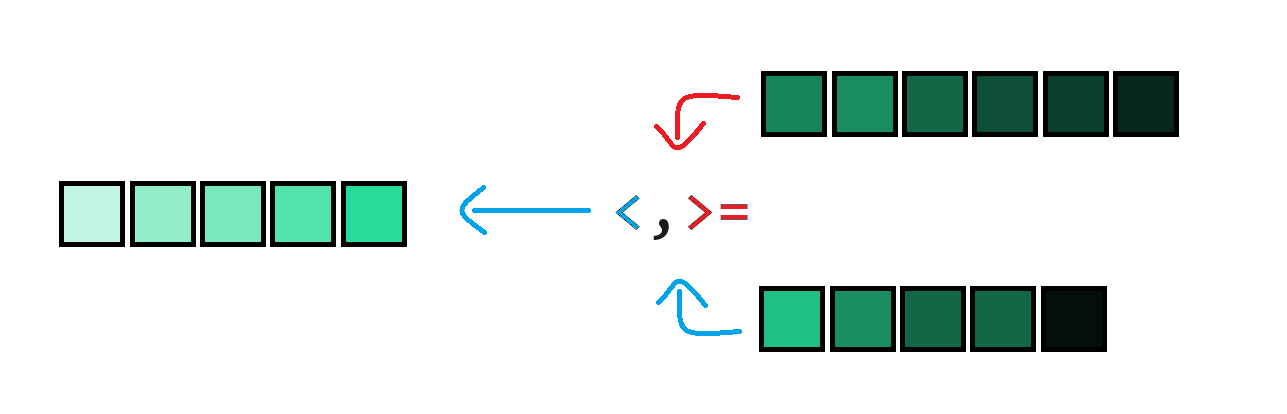
\includegraphics[width=10cm]{merge}
\end{center}

\textit{Důkaz:} Zkonstruovaná posloupnost je nutně seřazená, protože v každém kroku se odebírá minimum ze zbývajících prvků. Protože jsou vstupní posloupnosti seřazené, lze nalézt nejmenší prvek v posloupnostech v čase $\mathcal{O}(1)$ a algoritmus nepřekročí $n$ porovnání, protože po každém porovnání se odebere alespoň jeden prvek. Algoritmus skutečně pracuje v čase $\mathcal{O}(n)$.

\qed

\newpage

\subsection{Řešení}

\textbf{Vstup:} $k$ seřazených posloupností o celkem $n$ prvcích

\textbf{Výstup:} jedna seřazená posloupnost z původních prvků

V prvním kroku se posloupnosti rozdělí do $\lceil \frac{k}{2} \rceil$ dvojic. Dvojice se sloučí popsaným algoritmem do jedné větší seřazené posloupnosti. V případě lichého počtu je jedna posloupnost sama ve dvojici a je automaticky `sloučená'. Krok se opakuje, dokud nezbyde jedna seřazená posloupnost.

\begin{center}
    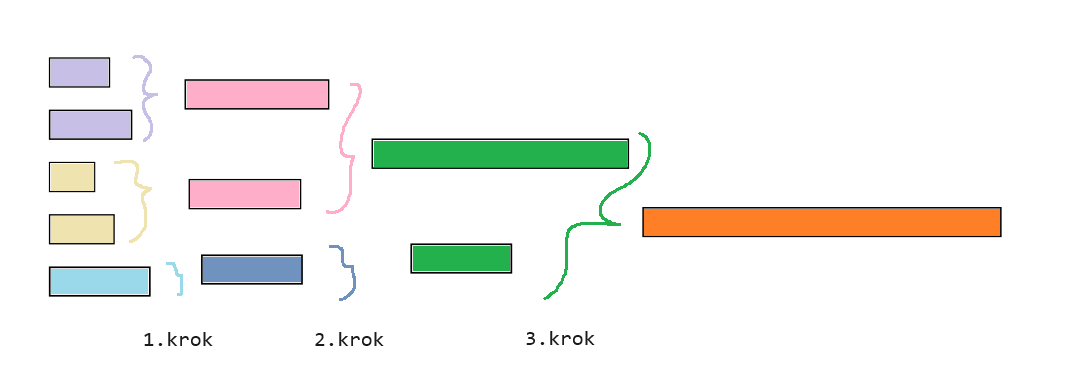
\includegraphics[width=12cm]{join}
\end{center}

V každém kroku dojde ke snížení počtu $l$ nesloučených posloupností o polovinu na počet vytvořených dvojic $\lceil \frac{l}{2} \rceil$ (počet potřebných sloučení se půlí). Počáteční počet posloupností je $k$, proto je potřeba $\lceil \log k \rceil$ kroků. V každém kroku se slučují posloupnosti, které mají celkem $n$ prvků, proto nám stačí maximálně $n$ operací na sloučení všech dvojic.

Ke sloučení je tedy zapotřebí $\lceil \log k \rceil$ kroků a v každém kroku nanejvýš $n$ operací. Algoritmus tedy pracuje v čase $\mathcal{O}(n \log k)$.

\qed

\end{document}
